\chapter{System Design and Methodology}

This chapter details the proposed architecture and implementation strategy of the agentic AI framework designed to support multi-cloud architectural decision-making. It outlines the constructive research methodology, system domain specifics, agentic architecture, key algorithms, and the tools and technologies employed.

\section{Research Design}

The research methodology follows a constructive research approach, also known as design science, where a novel artifact is systematically designed, implemented, and empirically evaluated to address a practical problem—in this case, cloud architecture recommendation and validation. This approach emphasizes iterative cycles of design, software development, and quantitative/qualitative assessment. In the context of this thesis, the constructive artifact is the Agentic AI Framework, and the empirical evaluation is conducted using the quantitative NLP metrics detailed in Chapter 5.

\section{System Domain: Multi-Cloud Environment (AWS and Azure)}

The system domain covers the two leading public cloud providers: Amazon Web Services (AWS) and Microsoft Azure. Both vendors expose hundreds of interrelated services that frequently overlap in purpose but differ in API design, pricing structures, and operational characteristics. A containerised compute workload, for instance, can target Amazon ECS or EKS on AWS, or Azure Container Apps and AKS on Azure; the choice involves tradeoffs that cannot be resolved by generic documentation lookup.

Within the framework, agents are structured around four canonical architecture domains present in both providers:

\begin{itemize}
    \item \textbf{Compute:} AWS services (EC2, Lambda, ECS, EKS, Auto Scaling) and Azure equivalents (Virtual Machines, Azure Functions, AKS, Container Apps, VM Scale Sets).
    \item \textbf{Network:} AWS constructs (VPC, Subnets, ALB, CloudFront, Route 53, Security Groups) and Azure counterparts (VNet, Application Gateway, Azure Front Door, Azure DNS, NSGs).
    \item \textbf{Storage:} AWS offerings (S3, EBS, EFS, Glacier) and Azure equivalents (Blob Storage, Managed Disks, Azure Files, Archive Storage).
    \item \textbf{Database:} AWS services (RDS, DynamoDB, ElastiCache) and Azure services (Azure SQL, Cosmos DB, Azure Cache for Redis, Azure Database for PostgreSQL).
\end{itemize}

All vendor-specific service names, validation checklists, and Infrastructure-as-Code resource identifiers are managed through an immutable \texttt{ProviderMeta} dataclass registry described further in Chapter 4. This decouples cloud-specific knowledge from the agent and graph logic, meaning that adding a third provider requires only a new registry entry rather than changes to the orchestration code.

\section{System Architecture}

The framework is realised as a cyclic state machine graph orchestrated via LangGraph \cite{langgraph2024docs}. Unlike Phase 1, where individual agent nodes were wired directly into the top-level graph, Phase 2 adopts a \textit{subgraph composition} pattern: the architect and validator phases are each compiled as independent \texttt{StateGraph} instances and then embedded as single nodes in the parent graph. This change yields a cleaner separation of concerns and allows each subgraph to be tested or extended in isolation.

The top-level topology is:

\begin{verbatim}
START
  |
  v
architect_phase  (subgraph)
  |
  v
validator_phase  (subgraph)
  |
  v
 [iteration_condition]
  |-- iterate --> architect_phase
  |-- finish  --> final_architecture_generator
                         |
                         v
                        END
\end{verbatim}

\begin{figure}[h]
  \begin{center}
  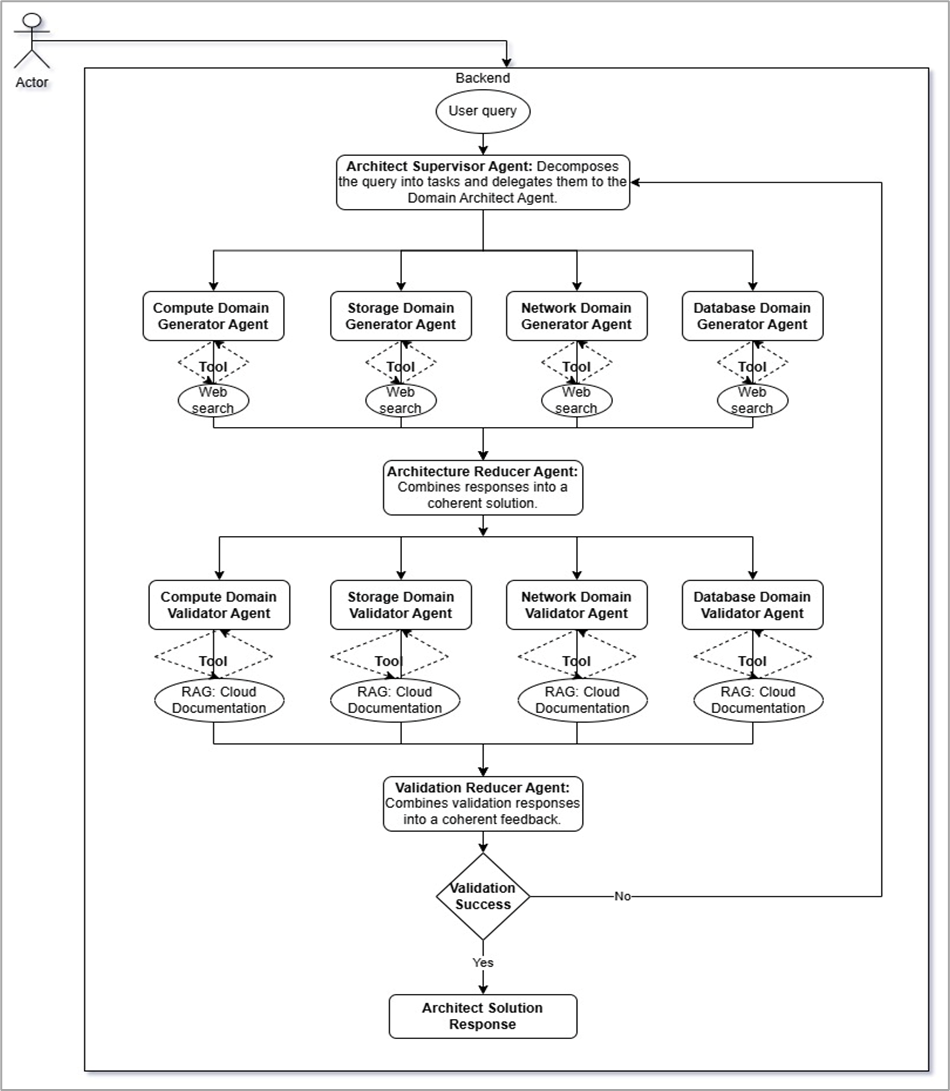
\includegraphics[width=11cm, height=12cm]{AgenticArchitect.png}
  \caption{Agent Framework: System Architecture Design}
  \label{fig:system_arch}
  \end{center}
\end{figure}

Each subgraph internally follows a fan-out/fan-in structure: a supervisor node decomposes the problem, four domain agent nodes execute in parallel, and a synthesizer node aggregates their outputs before the subgraph returns control to the parent graph. The architecture operates across six conceptual phases:

\subsection{Phase 1: Query Decomposition}

The \textbf{Architect Supervisor Agent} receives the user's natural-language problem statement and decomposes it into four structured domain tasks via a call to a \texttt{with\_structured\_output(TaskDecomposition)} LLM. Each task carries a precise description, key requirements, and expected deliverables. When running in a refinement iteration, the supervisor also receives the previous cycle's validation feedback and adjusts task definitions accordingly.

\subsection{Phase 2: Generation}

Four \textbf{Domain Architect Agents} (compute, network, storage, database) execute concurrently. Each agent operates a bounded ReAct loop \cite{yao2023react} equipped with two tools: a \textbf{Web Search} capability backed by the Google Serper API for real-time information, and a \textbf{RAG Search} capability backed by a provider-specific ChromaDB vector store. A configurable maximum number of tool-call rounds prevents unbounded token consumption.

\subsection{Phase 3: Architecture Synthesis}

The \textbf{Architect Synthesizer} waits for all four domain outputs and merges them into a single coherent architecture proposal. It resolves any cross-domain incompatibilities (for example, ensuring the network configuration exposes the correct ports for the proposed compute services) and produces both a structured component dictionary and a human-readable summary.

\subsection{Phase 4: Validation with Reranked RAG}

The \textbf{Validator Supervisor Agent} inspects the synthesized components and assigns targeted validation tasks to four \textbf{Domain Validator Agents}. Each validator exclusively uses the RAG tool, not web search, so that fact-checking is grounded in the curated documentation corpus rather than the open internet. Within the RAG tool, a two-stage retrieval protocol operates: ChromaDB performs an initial embedding-similarity search over a larger candidate pool (top-$k \times$ multiplier documents), and a FlashRank cross-encoder \cite{gao2023retrieval} subsequently rescores these candidates and returns only the top-$k$ highest-relevance passages.

\subsection{Phase 5: Validation Synthesis and Iteration}

The \textbf{Validation Synthesizer} consolidates domain-level feedback into a global assessment. The \texttt{iteration\_condition} function then inspects the state: if the minimum iteration count has not been reached, or if factual errors were reported and the maximum has not been exceeded, the graph routes back to the architect phase. Otherwise it routes to the final generator. This conditional edge is the mechanism that implements the Evaluator-Optimizer loop from Phase 1 \cite{anthropic2024agents}, now operating over subgraphs.

\subsection{Phase 6: Final Architecture Generation}

Once iteration terminates, the \textbf{Final Architecture Generator} compiles a deployment-ready document covering executive summary, domain-specific specifications, security controls, cost optimisation strategies, and Infrastructure-as-Code guidance. This output is persisted in the LangGraph state and returned to the UI or CLI caller.

\section{Model Selection Subsystem}

A persistent limitation of fixed-model architectures is that no single LLM dominates across all tasks: high-capability reasoning models process complex decomposition better, but their cost per token can be prohibitive for repetitive domain agent calls. Phase 2 introduces a two-tier model selection system.

A central model catalog defines available models across three providers (OpenAI GPT-5.4 family, Anthropic Claude~4.6 family, Google Gemini~3.1/2.5 family), tagged by tier (reasoning or execution). The \texttt{RuntimeContext} carries a base reasoning LLM and a base execution LLM set at service startup. Per-run overrides carried in the LangGraph state allow the UI to nominate different models for individual requests without restarting the server. Helper functions \texttt{resolve\_reasoning\_llm} and \texttt{resolve\_execution\_llm} transparently resolve this precedence, ensuring that supervisors and synthesizers always use the appropriate reasoning-tier model while domain agents use the more cost-efficient execution-tier model.

\section{Algorithms and Techniques}

\subsection{Core Workflow: Evaluator-Optimizer}

The central workflow is a self-correcting Evaluator-Optimizer loop depicted in Figure \ref{fig:eval_workflow}, inspired by \cite{anthropic2024agents}. In each iteration, the architect phase proposes an architecture, the validator phase critiques it with reranked RAG, and the conditional routing edge decides whether to continue or finalise.

\begin{figure}[h]
    \centering
    \fbox{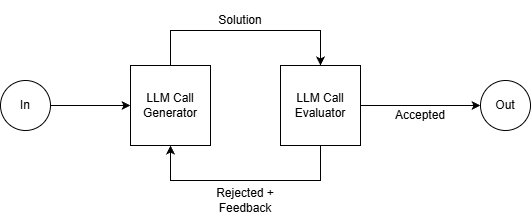
\includegraphics[width=0.9\textwidth]{Evalutor-Optimiser.drawio.png}}
    \caption[The Evaluator-Optimizer Workflow]{The Evaluator-Optimizer Workflow (Source: Adapted from \cite{anthropic2024agents})}
    \label{fig:eval_workflow}
\end{figure}

\subsection{Knowledge Base Construction}

A robust multi-provider knowledge base underpins RAG validation, constructed in four stages:

\begin{enumerate}
    \item \textbf{Data Collection:} AWS documentation is aggregated via automated web scraping of official AWS URLs, supplemented by manual review for services with non-standard documentation layouts. Azure documentation is ingested using \texttt{git sparse-checkout} against Microsoft's public GitHub documentation repository, avoiding scraping constraints while ensuring currency.
    \item \textbf{Document Parsing:} The Docling toolkit \cite{docling2025paper, docling2024web} converts PDFs and DOCX whitepapers to cleaned Markdown, stripping non-vectorisable elements such as decorative images and formatting tables.
    \item \textbf{Embedding Generation:} The \texttt{nomic-embed-text} model served locally via Ollama~\cite{ollama2024web} produces dense vector embeddings on Apple Silicon using Metal Performance Shaders \cite{apple2024mps} for local throughput.
    \item \textbf{Vector Indexing:} ChromaDB \cite{chromadb2024} maintains separate, persistently stored collections for AWS and Azure documentation, keyed by provider name. At query time, FlashRank cross-encoder reranking further filters the retrieved candidates before they reach the validator agent.
\end{enumerate}

\section{Tools and Technologies}

The system employs the following core technologies:

\begin{itemize}
    \item \textbf{Programming Language:} Python 3.11+ with typed modules and pydantic-settings.
    \item \textbf{Frontend Framework:} Next.js 15 with React 18 and the \texttt{@xyflow/react} library for interactive workflow graph visualization.
    \item \textbf{LLM Models:} Three provider families are available: OpenAI GPT-5.4 / GPT-5.4 Mini / GPT-5.4 Nano; Anthropic Claude Opus 4.6 / Claude Sonnet 4.6 / Claude Haiku 4.5; Google Gemini 3.1 Pro / Gemini 3 Flash / Gemini 2.5 Flash. Supervisors and synthesisers default to the reasoning tier; domain agents use the execution tier.
    \item \textbf{Agentic Framework:} LangGraph \cite{langgraph2024docs} with subgraph composition for modular architect and validator workflows.
    \item \textbf{LLM Orchestration:} LangChain \cite{langchain2024docs} and LCEL \cite{langchain2024lcel} for prompt management, tool binding, and structured output parsing.
    \item \textbf{Embedding and Vector Store:} Ollama \cite{ollama2024web} with \texttt{nomic-embed-text}, persisted in provider-scoped ChromaDB collections \cite{chromadb2024}.
    \item \textbf{Reranking:} FlashRank with the \texttt{ms-marco-MiniLM-L-12-v2} cross-encoder model for two-stage retrieval quality improvement.
    \item \textbf{Hardware Acceleration:} Apple Metal Performance Shaders (MPS) \cite{apple2024mps} for local embedding generation on Apple Silicon.
    \item \textbf{Observability:} LangSmith for end-to-end trace inspection across the cyclic multi-agent workflow.
\end{itemize}

